\section{Score Addressability}\label{sec:score_addressability}


\begin{comment}
Score Addressability [Trevor]
    - Iteration
        - methods that "get_*"
            Container.select_leaves
            Container.select_notes_and_chords
            IterationAgent.by_class, .by_logical_tie, .by_timeline, .by_vertical_moment, .depth_first
        - efficient and intuitive navigation of the score hierarchy does what mapping does in a functional program
            -containers partake of Python's sequence iterating interface (for loops work)
    - Structural Addressing
        - numeric addressing
        - temporal addressing
        - named addressing
\end{comment}

\subsection{Addressing objects by index}

Abjad allows the numeric addressing of all score components. Abjad score
components are zero-indexed from the start of the container which holds them:
the statement \texttt{staff[0]} addresses the first component contained in
\texttt{staff} while the statement \texttt{staff[1]} addresses the component
after that, and so on. Negative indices address components from the end of the
container which holds them. Python's slice notation may be used to retrieve an
arbitrary number of contiguous components at one time. As an example of the
latter, the statement \texttt{staff[15:25]} selects the ten components in
\texttt{staff} between indices 15 and 25. The conventions of Abjad's numeric
addressing regime follow those of Python's list and tuple interface exactly. 

\begin{lstlisting}
>>> staff_group = score[0]
\end{lstlisting}


\begin{lstlisting}
>>> upper_staff = score[0][0]
\end{lstlisting}


\begin{lstlisting}
>>> first_tuplet = score[0][0][0]
>>> show(first_tuplet)
\end{lstlisting}

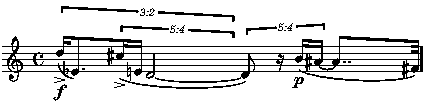
\includegraphics[scale=1.0]{images/score_addressability-1.pdf}


\subsection{Addressing objects temporally}

Here is some text.

A \emph{timespan} is an object-oriented model of a start/stop offset pair.
Abjad's \texttt{Timespan} class affords users with a variety of tests for
relationships between timespans such as overlap and intersection.

All durated objects in Abjad have a timespan, including all score components
and spanners, allowing them to partake in timespan-based relationship modeling
without regard for hierarchical score structure.

\subsection{Addressing objects by name}

Here is some text.

\begin{lstlisting}
>>> upper_staff = score['Upper Staff']
>>> show(upper_staff)
\end{lstlisting}

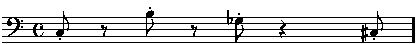
\includegraphics[scale=1.0]{images/score_addressability-2.pdf}


\begin{lstlisting}
>>> lower_staff = score['Lower Staff']
>>> show(lower_staff)
\end{lstlisting}

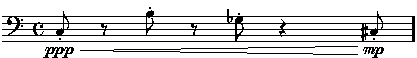
\includegraphics[scale=1.0]{images/score_addressability-3.pdf}


\subsection{Iterating throught score}

Here is some text.

\begin{lstlisting}
>>> for x in score['Upper Staff']:
...     x
... 
Tuplet(Multiplier(2, 3), 'd\'\'16 ef\'8. Tuplet(Multiplier(4, 5), "cs\'\'16 e\'16 d\'2 ~")')
Tuplet(Multiplier(4, 5), "d'8 r16 b'16 as'16 ~")
Note("as'8..")
Note("fs'32")
\end{lstlisting}


\begin{lstlisting}
>>> for component in iterate(score).by_timeline():
...     component
... 
Note("d''16")
Note('c8')
Note("ef'8.")
Rest('r8')
Note("cs''16")
Note("e'16")
Note("d'2")
Note('b8')
Rest('r8')
Note("d'8")
Note('gf8')
Rest('r16')
Rest('r4')
Note("b'16")
Note("as'16")
Note("as'8..")
Note('cs8')
Note("fs'32")
\end{lstlisting}


\begin{lstlisting}
>>> for logical_tie in iterate(score).by_logical_tie(
...     nontrivial=True,
...     pitched=True,
...     ):
...     logical_tie
... 
LogicalTie(Note("d'2"), Note("d'8"))
LogicalTie(Note("as'16"), Note("as'8.."))
\end{lstlisting}

